\documentclass[11pt]{article}
\usepackage{graphicx}
\usepackage{hyperref}
\usepackage{natbib}

\setlength{\textwidth}{6.5in}
\setlength{\headheight}{0in}
\setlength{\textheight}{8.0in}
\setlength{\hoffset}{0in}
\setlength{\voffset}{0in}
\setlength{\oddsidemargin}{0in}
\setlength{\evensidemargin}{0in}

\title{CP PS1}
  
\author{Shadi Ali Ahmad}


\begin{document}

\maketitle

\abstract{This is Shadi's LaTeX PS1 submission for Professor Blanton's Computational Physics first problem set during Fall 2023. My GitHub account name is shadi-r-aa.}

\section{Computing background}
\label{sec:bg}
I have coded minimally during college, and the most I have done is produce pretty plots for some of my papers using Mathematica.

\section{Goals}
\label{sec:gl}

 I am looking forward to learning more about computing, especially since I am interested in complexity classes and would like to understand them at a deeper level. I would also like to get better at numerical integration and simulations, as many times in my research, it is almost impossible to get an analytic expression for some problems.

\section{Plans}
My future plan, for now, is to remain in academia. 
\section{Gaussian plot}
\begin{figure}[h!]
\centering
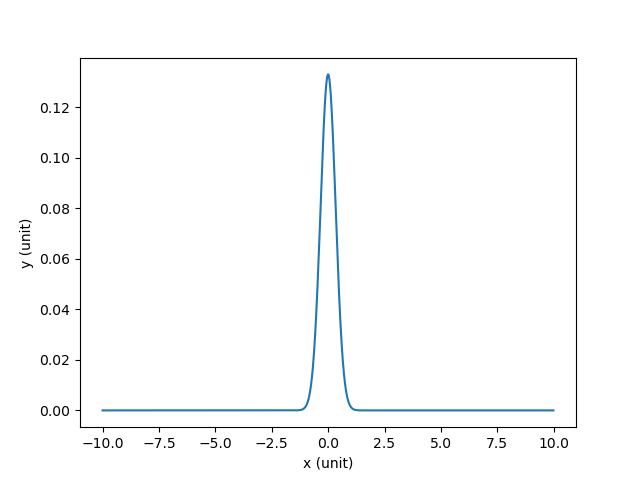
\includegraphics[width=0.8\textwidth]{gaussian.png}
\caption{ \label{fig:example} A Gaussian $y(x)$ with zero mean and a standard deviation of $3$ is shown across the range $x\in [-10,10]$. }
\end{figure}



\bibliographystyle{apj}
\bibliography{example}

\end{document}

 
 
